%======================================================
% AGENTIC DOCUMENT PROCESSOR — PRESENTATION
% Compile with: pdflatex presentation.tex  (twice for refs)
% Or upload to Overleaf for instant PDF
%======================================================
\documentclass[aspectratio=169,t]{beamer}

%-------- Theme & Colors --------
\usetheme{Madrid}
\usecolortheme{whale}
\setbeamertemplate{navigation symbols}{}
\setbeamertemplate{footline}[frame number]
\setbeamerfont{title}{size=\Large,series=\bfseries}
\setbeamerfont{frametitle}{size=\normalsize,series=\bfseries}

%-------- Packages --------
\usepackage[utf8]{inputenc}
\usepackage[T1]{fontenc}
\usepackage{lmodern}
\usepackage{graphicx}
\usepackage{booktabs}
\usepackage{colortbl}
\usepackage{xcolor}
\usepackage{tikz}
\usepackage{pgfplots}
\pgfplotsset{compat=1.18}
\usepackage{listings}
\usepackage{fontawesome5}
\usepackage{multicol}
\usepackage{tcolorbox}
\tcbuselibrary{skins,breakable}
\usepackage{array}
\usepackage{makecell}
\usepackage{newunicodechar}
\newunicodechar{→}{\ensuremath{\rightarrow}}
\newunicodechar{←}{\ensuremath{\leftarrow}}
\newunicodechar{—}{---}
\newunicodechar{–}{--}
\newunicodechar{…}{...}
\usetikzlibrary{shapes.geometric, arrows.meta, positioning, fit, backgrounds, shadows, decorations.pathreplacing}

%-------- Color Palette --------
\definecolor{primary}{RGB}{25,85,160}
\definecolor{secondary}{RGB}{0,140,200}
\definecolor{accent}{RGB}{255,140,0}
\definecolor{success}{RGB}{46,160,67}
\definecolor{danger}{RGB}{211,47,47}
\definecolor{lightgray}{RGB}{245,245,250}
\definecolor{darkgray}{RGB}{50,50,60}
\definecolor{groqcolor}{RGB}{120,50,180}
\definecolor{bedrockcolor}{RGB}{35,135,80}
\definecolor{codegreen}{RGB}{50,150,50}
\definecolor{codepurple}{RGB}{130,0,180}
\definecolor{codegray}{RGB}{100,100,100}

\setbeamercolor{palette primary}{bg=primary}
\setbeamercolor{palette secondary}{bg=secondary}
\setbeamercolor{palette quaternary}{bg=primary}
\setbeamercolor{title}{fg=white}
\setbeamercolor{block title}{bg=primary,fg=white}
\setbeamercolor{alerted text}{fg=accent}

%-------- Code Listings --------
\lstset{
  basicstyle=\ttfamily\scriptsize,
  keywordstyle=\color{primary}\bfseries,
  stringstyle=\color{codegreen},
  commentstyle=\color{codegray}\itshape,
  numberstyle=\tiny\color{codegray},
  numbers=left,
  stepnumber=1,
  showstringspaces=false,
  breaklines=true,
  frame=single,
  rulecolor=\color{secondary!40},
  backgroundcolor=\color{lightgray},
  tabsize=2,
  language=Python,
  xleftmargin=1em,
  xrightmargin=0.5em,
  literate=
    {->}{{$\rightarrow$}}2
    {→}{{$\rightarrow$}}1
    {—}{{---}}1
    {–}{{--}}1
    {…}{{...}}1,
}

%-------- TColorBox Styles --------
\tcbset{
  mybox/.style={
    enhanced, colback=lightgray, colframe=primary,
    fonttitle=\bfseries\small, coltitle=white, attach boxed title to top left,
    boxed title style={colback=primary, rounded corners=all},
    sharp corners, boxrule=0.5pt, left=4pt, right=4pt, top=6pt
  },
}

%-------- Title Slide Info --------
\title[Agentic Doc Processor]{\textbf{Agentic Document Processor}\\[4pt]
\large Local Pipeline with LangGraph + Amazon Bedrock}
\subtitle{Prototype 2 — Intelligent Document Ingestion, Extraction, Validation \& Redaction}
\author{\textbf{Presented by: [Your Name]}}
\institute{Agentic AI Systems — Capstone Project}
\date{February 2026}

%======================================================
\begin{document}
%======================================================

%-------- TITLE FRAME --------
\begin{frame}[plain]
\begin{tikzpicture}[remember picture, overlay]
  % Background gradient bar
  \fill[primary] (current page.north west) rectangle ([yshift=-2.2cm]current page.north east);
  \fill[secondary!80] ([yshift=-2.2cm]current page.north west) rectangle ([yshift=-2.5cm]current page.north east);
  \fill[accent] ([yshift=-2.5cm]current page.north west) rectangle ([yshift=-2.6cm]current page.north east);
  % Bottom strip
  \fill[primary!90] (current page.south west) rectangle ([yshift=0.7cm]current page.south east);
\end{tikzpicture}

\vspace{0.4cm}
\begin{center}
  {\color{white}\fontsize{22}{26}\selectfont\bfseries Agentic Document Processor}\\[6pt]
  {\color{white!80}\fontsize{13}{16}\selectfont Local Pipeline · LangGraph · Amazon Bedrock}\\[10pt]
  \color{accent}\rule{10cm}{1.5pt}\\[8pt]
  {\color{white}\small Prototype 2 — Intelligent Document Ingestion, Classification, Extraction,\\
  Validation, PII Redaction \& Responsible AI Reporting}
\end{center}
\vspace{0.5cm}
\begin{center}
  
\begin{tikzpicture}
    \node[fill=white, rounded corners=6pt, inner sep=6pt, draw=accent, line width=1.2pt] {
      \footnotesize\color{primary}
      \faCode~LangGraph \quad
      \faCloud~Bedrock Claude 3.5 Haiku \quad
      \faRobot~Multi-Agent \quad
      \faShieldAlt~PII Redaction \quad
      \faChartBar~Responsible AI
    };
  \end{tikzpicture}
\end{center}
\vspace{0.3cm}
{\color{white!60}\centering\tiny February 2026 | Capstone Project Presentation}
\end{frame}

%-------- AGENDA --------
\begin{frame}{Agenda}
\begin{columns}[T]
\column{0.48\textwidth}
\begin{tcolorbox}[mybox, title={\faList~Presentation Flow}]
\begin{enumerate}\setlength\itemsep{5pt}
  \item[\textcolor{accent}{\bfseries 1.}] \textbf{Problem Statement}\\
       {\scriptsize Scope, pain points, industry need}
  \item[\textcolor{accent}{\bfseries 2.}] \textbf{Solution Overview}\\
       {\scriptsize What we built and why}
  \item[\textcolor{accent}{\bfseries 3.}] \textbf{Tech Stack}\\
       {\scriptsize Tools, frameworks, providers}
  \item[\textcolor{accent}{\bfseries 4.}] \textbf{High-Level Architecture}\\
       {\scriptsize Data flow \& agent orchestration}
  \item[\textcolor{accent}{\bfseries 5.}] \textbf{Deep Dive: Codebase}\\
       {\scriptsize File-by-file walkthrough}
\end{enumerate}
\end{tcolorbox}

\column{0.48\textwidth}
\begin{tcolorbox}[mybox, title={\faChartLine~Evaluation \& Demo}]
\begin{enumerate}\setlength\itemsep{5pt}
  \item[\textcolor{accent}{\bfseries 6.}] \textbf{Evaluation Metrics}\\
       {\scriptsize Accuracy, PII, latency results}
  \item[\textcolor{accent}{\bfseries 7.}] \textbf{Salient Features}\\
       {\scriptsize What makes it stand out}
  \item[\textcolor{accent}{\bfseries 8.}] \textbf{Responsible AI}\\
       {\scriptsize Trace logs, auditability}
  \item[\textcolor{accent}{\bfseries 9.}] \textbf{Live Demo}\\
       {\scriptsize Streamlit UI + API}
  \item[\textcolor{accent}{\bfseries 10.}] \textbf{Future Scope}\\
       {\scriptsize Roadmap \& extensions}
\end{enumerate}
\end{tcolorbox}
\end{columns}
\end{frame}

%======================================================
\section{Problem Statement}
%======================================================

\begin{frame}{Problem Statement}
\begin{tcolorbox}[enhanced, colback=danger!6, colframe=danger, sharp corners, boxrule=1pt,
  title={\faExclamationTriangle~The Core Problem}, fonttitle=\bfseries, coltitle=white]
\textbf{Organizations receive thousands of heterogeneous documents daily} — invoices, resumes, medical records, contracts, IDs, transcripts — and must manually classify, extract, validate, and redact sensitive data. This is:
\begin{itemize}
  \item \textbf{Slow}: Human reviewers process 10–50 docs/day vs thousands needed
  \item \textbf{Error-prone}: ~30\% field extraction error rate in manual processes
  \item \textbf{Privacy risk}: PII leaks in downstream systems without systematic redaction
  \item \textbf{Non-auditable}: No structured trace of who/what acted on each document
\end{itemize}
\end{tcolorbox}

\vspace{6pt}
\begin{columns}[T]
\column{0.3\textwidth}
\begin{tcolorbox}[enhanced, colback=accent!10, colframe=accent, sharp corners, boxrule=0.8pt]
\centering\small\textbf{\faFileAlt~Document Chaos}\\[4pt]
\scriptsize PDFs, images, DOCX, TXT in 6+ categories with zero labeling
\end{tcolorbox}
\column{0.3\textwidth}
\begin{tcolorbox}[enhanced, colback=accent!10, colframe=accent, sharp corners, boxrule=0.8pt]
\centering\small\textbf{\faLock~PII Exposure}\\[4pt]
\scriptsize SSN, Aadhaar, emails, DOBs flow unmasked into analytics pipelines
\end{tcolorbox}
\column{0.3\textwidth}
\begin{tcolorbox}[enhanced, colback=accent!10, colframe=accent, sharp corners, boxrule=0.8pt]
\centering\small\textbf{\faExclamationCircle~No Auditability}\\[4pt]
\scriptsize GDPR/HIPAA require decision traces — manual processes leave no log
\end{tcolorbox}
\end{columns}
\end{frame}

\begin{frame}{Problem Scope \& Industry Need}
\begin{columns}[T]
\column{0.55\textwidth}
\textbf{Document Types in Scope:}
\vspace{4pt}

\begin{tabular}{@{}lll@{}}
\toprule
\rowcolor{primary!15}
\textbf{Type} & \textbf{Key Fields} & \textbf{PII Risk} \\
\midrule
\faReceipt~Financial & Amounts, invoices & Low \\
\faUser~Resume & Name, email, phone & \textcolor{danger}{High} \\
\faBriefcase~Job Offer & Salary, dates & Medium \\
\faNotesMedical~Medical & Diagnosis, DOB & \textcolor{danger}{Critical} \\
\faIdCard~Identity & ID\#, DOB, address & \textcolor{danger}{Critical} \\
\faGraduationCap~Academic & GPA, student ID & Medium \\
\bottomrule
\end{tabular}

\vspace{8pt}
\textbf{Regulatory Drivers:}
\begin{itemize}\scriptsize
  \item \textbf{GDPR} — right to erasure, data minimization
  \item \textbf{HIPAA} — PHI protection in medical docs
  \item \textbf{India DPDP Act 2023} — Aadhaar, PAN masking required
\end{itemize}

\column{0.42\textwidth}
\begin{tcolorbox}[mybox, title={\faBullseye~Success Criteria}]
\begin{itemize}\small\setlength\itemsep{4pt}
  \item[\textcolor{success}{\faCheckCircle}] Extraction accuracy $\geq$ \textbf{90\%}
  \item[\textcolor{success}{\faCheckCircle}] PII Recall $\geq$ \textbf{95\%}
  \item[\textcolor{success}{\faCheckCircle}] PII Precision $\geq$ \textbf{90\%}
  \item[\textcolor{success}{\faCheckCircle}] Workflow success $\geq$ \textbf{90\%}
  \item[\textcolor{success}{\faCheckCircle}] P95 latency $\leq$ \textbf{4 seconds}
  \item[\textcolor{success}{\faCheckCircle}] Graceful LLM retry/fallback
  \item[\textcolor{success}{\faCheckCircle}] Full Responsible AI audit log
\end{itemize}
\end{tcolorbox}
\end{columns}
\end{frame}

%======================================================
\section{Solution Overview}
%======================================================

\begin{frame}{Our Solution — What \& Why}
\begin{tcolorbox}[enhanced, colback=success!6, colframe=success, sharp corners, boxrule=1pt,
  title={\faRocket~Solution: Agentic Document Processor}, fonttitle=\bfseries, coltitle=white]
\textbf{A local, production-grade agentic pipeline} that ingests any document, runs it through 6 specialized AI agents orchestrated by LangGraph, and produces validated JSON + redacted output with a full Responsible AI audit trail.
\end{tcolorbox}

\vspace{8pt}
\begin{columns}[T]
\column{0.48\textwidth}
\textbf{\faQuestion~Why LangGraph?}
\begin{itemize}\small
  \item \textbf{Stateful graph} — every agent reads/writes one shared \texttt{DocumentState} object
  \item \textbf{Conditional routing} — self-repair fires only when accuracy $<$ 80\%
  \item \textbf{Checkpointing} — \texttt{MemorySaver} persists state mid-pipeline
  \item \textbf{Visual} — auto-generates Mermaid diagram of the graph
\end{itemize}

\column{0.48\textwidth}
\textbf{\faQuestion~Why Amazon Bedrock + Groq?}
\begin{itemize}\small
  \item \textbf{Groq} — primary LLM, 300+ tokens/sec, $<$1.5s latency
  \item \textbf{Bedrock Claude 3.5 Haiku} — reliable fallback with AWS SLA
  \item \textbf{HuggingFace API} — tertiary fallback
  \item \textbf{Local phi-2} — offline last resort (no API dependency)
\end{itemize}
\end{columns}
\end{frame}

%======================================================
\section{Tech Stack}
%======================================================

\begin{frame}{Technology Stack}
\begin{columns}[T]
\column{0.32\textwidth}
\begin{tcolorbox}[mybox, title={\faCode~Core Framework}]
\begin{itemize}\scriptsize\setlength\itemsep{3pt}
  \item \textbf{Python 3.11}
  \item \textbf{LangGraph} — agent orchestration
  \item \textbf{LangChain} — document loaders
  \item \textbf{Pydantic v2} — schema validation
  \item \textbf{FastAPI} — REST API
  \item \textbf{Streamlit} — UI dashboard
\end{itemize}
\end{tcolorbox}

\column{0.32\textwidth}
\begin{tcolorbox}[mybox, title={\faCloud~LLM Providers}]
\begin{itemize}\scriptsize\setlength\itemsep{3pt}
  \item \textcolor{groqcolor}{\textbf{Groq}} — llama-3.1-8b-instant
  \item \textcolor{bedrockcolor}{\textbf{Bedrock}} — Claude 3.5 Haiku
  \item \textbf{HuggingFace} — Llama 3.1
  \item \textbf{Local phi-2} — offline fallback
  \item \textbf{Tenacity} — retry/backoff
\end{itemize}
\end{tcolorbox}

\column{0.32\textwidth}
\begin{tcolorbox}[mybox, title={\faShieldAlt~Data \& Privacy}]
\begin{itemize}\scriptsize\setlength\itemsep{3pt}
  \item \textbf{Presidio} — PII detection engine
  \item \textbf{spaCy} — NLP entity recognition
  \item \textbf{Tesseract OCR} — image text extraction
  \item \textbf{PyPDF2 / pdf2image} — PDF parsing
  \item \textbf{structlog} — structured JSON logging
  \item \textbf{FAISS} — optional vector lookup
\end{itemize}
\end{tcolorbox}
\end{columns}

\vspace{6pt}
\begin{center}
\begin{tikzpicture}
  \node[fill=primary!10, draw=primary, rounded corners=5pt, inner sep=5pt, font=\scriptsize] {
    \faPython~Python 3.11 \quad
    \faProjectDiagram~LangGraph \quad
    \faCloud~Bedrock \quad
    \faShieldAlt~Presidio \quad
    \faEye~Tesseract \quad
    \faServer~FastAPI \quad
    \faDesktop~Streamlit \quad
    \faFlask~Pytest
  };
\end{tikzpicture}
\end{center}
\end{frame}

%======================================================
\section{High-Level Architecture}
%======================================================

\begin{frame}{High-Level Architecture — Data Flow}
\centering
\resizebox{0.96\textwidth}{!}{%
\begin{tikzpicture}[
  node distance=1.5cm,
  agent/.style={rectangle, rounded corners=8pt, minimum width=2.4cm, minimum height=0.95cm,
    text centered, draw=primary, fill=secondary!12, font=\small\bfseries, text width=2.4cm,
    drop shadow={shadow xshift=1.5pt, shadow yshift=-1.5pt, fill=black!15}},
  io/.style={rectangle, rounded corners=5pt, minimum width=2cm, minimum height=0.8cm,
    text centered, draw=darkgray, fill=lightgray, font=\scriptsize, text width=2.2cm},
  decision/.style={diamond, minimum width=2.2cm, minimum height=1.1cm,
    text centered, draw=accent, fill=accent!15, font=\scriptsize\bfseries, aspect=2},
  llm/.style={rectangle, rounded corners=4pt, minimum width=2cm, minimum height=0.7cm,
    text centered, draw=groqcolor, fill=groqcolor!10, font=\scriptsize, text width=2.2cm},
  flow/.style={->, >=Stealth, thick, draw=primary!70},
  backflow/.style={->, >=Stealth, thick, draw=accent, dashed},
  lflow/.style={->, >=Stealth, thin, draw=groqcolor!60, dashed}
]

% Input
\node[io] (input) {\faFileAlt\\\textbf{Document}\\\tiny PDF/TXT/DOCX/IMG};

% Document Loader
\node[agent, right=1cm of input] (loader)
  {\faDownload\\Document\\Loader};

% Classifier
\node[agent, right=1.3cm of loader] (classify)
  {\faTags\\Classifier\\Agent};

% Extractor
\node[agent, right=1.3cm of classify] (extract)
  {\faCogs\\Extractor\\Agent};

% Validator
\node[agent, right=1.3cm of extract] (validate)
  {\faCheckDouble\\Validator\\Agent};

% Decision
\node[decision, right=1.3cm of validate] (decide)
  {Valid?};

% Self Repair (below decision)
\node[agent, below=1.2cm of decide] (repair)
  {\faWrench\\Self-Repair\\Node};

% Redactor
\node[agent, right=1.3cm of decide] (redact)
  {\faUserSecret\\Redactor\\Agent};

% Reporter
\node[agent, right=1.3cm of redact] (report)
  {\faChartBar\\Reporter\\Agent};

% Output
\node[io, right=1cm of report] (output)
  {\faFileCode\\\textbf{JSON Report}\\\tiny + Redacted Text};

% LLM Chain below agents
\node[llm, below=2.4cm of classify, xshift=0.6cm] (llm1)
  {\textcolor{groqcolor}{\textbf{Groq}} (Primary)};
\node[llm, right=0.3cm of llm1] (llm2)
  {\textcolor{bedrockcolor}{\textbf{Bedrock}} (Fallback)};
\node[llm, right=0.3cm of llm2] (llm3)
  {HuggingFace (Tertiary)};
\node[llm, right=0.3cm of llm3] (llm4)
  {Local phi-2 (Last resort)};

% State store
\node[io, below=0.5cm of repair, xshift=2.5cm] (state)
  {\faDatabase\\\textbf{DocumentState}\\\tiny LangGraph shared state};

% Flows
\draw[flow] (input) -- (loader);
\draw[flow] (loader) -- (classify);
\draw[flow] (classify) -- (extract);
\draw[flow] (extract) -- (validate);
\draw[flow] (validate) -- (decide);
\draw[flow] (decide) -- node[above,font=\scriptsize,text=success]{\faCheck~Yes} (redact);
\draw[backflow] (decide) -- node[right,font=\scriptsize,text=danger]{\faTimes~No} (repair);
\draw[backflow] (repair.west) -- +(-0.5,0) |- (validate.south) node[font=\scriptsize, pos=0.7, left, text=accent]{retry};
\draw[flow] (redact) -- (report);
\draw[flow] (report) -- (output);

% LLM arrows
\draw[lflow] (llm1.north) -- ++(0,0.4) -| (classify.south);
\draw[lflow] (llm1.north) -- ++(0,0.4) -| (extract.south);
\draw[lflow] (llm1.north) -- ++(0,0.4) -| (validate.south);
\draw[lflow] (llm1.north) -- ++(0,0.4) -| (repair.south);
\draw[lflow] (llm1.north) -- ++(0,0.4) -| (redact.south);

% Fallback arrows
\draw[lflow, draw=accent!50] (llm1) -- (llm2) node[above, font=\tiny, pos=0.5]{fallback};
\draw[lflow, draw=accent!50] (llm2) -- (llm3) node[above, font=\tiny, pos=0.5]{fallback};
\draw[lflow, draw=accent!50] (llm3) -- (llm4) node[above, font=\tiny, pos=0.5]{fallback};

\end{tikzpicture}
}
\end{frame}

\begin{frame}[fragile]{LangGraph State --- The Shared Backbone}
\begin{columns}[T]
\column{0.52\textwidth}
\textbf{\faDatabase~\texttt{DocumentState} (TypedDict)}\\[4pt]
{\scriptsize Defined in \texttt{graph/state.py} — single object passed between all nodes:}

\vspace{4pt}
\begin{tcolorbox}[enhanced, colback=lightgray, colframe=primary!50, sharp corners, boxrule=0.5pt]
\begin{lstlisting}[numbers=none, frame=none, backgroundcolor=\color{lightgray}]
class DocumentState(TypedDict):
  # Input
  file_path: str
  raw_text: str
  # Classification output
  doc_type: Optional[DocumentType]
  classification_result: ClassificationResult
  # Extraction output
  extracted_fields: Dict[str, Any]
  # Validation + repair triggers
  needs_repair: bool
  repair_attempts: int
  current_accuracy: float    # 0.0–1.0
  missing_schema_fields: List[str]
  # Redaction output
  redacted_text: str
  redaction_result: RedactionResult
  # Responsible AI
  trace_log: List[ResponsibleAILog]
  agent_timings: Dict[str, float]
  errors: List[str]
  success: bool
\end{lstlisting}
\end{tcolorbox}

\column{0.44\textwidth}
\textbf{\faProjectDiagram~Graph Topology}\\[6pt]

\begin{tcolorbox}[enhanced, colback=lightgray, colframe=primary!50, sharp corners, boxrule=0.5pt]
\begin{lstlisting}[numbers=none, frame=none, backgroundcolor=\color{lightgray}]
START
  +---> [classify]
          +---> [extract]
                  +---> [validate]
                          +-- Valid? --+
                          |           |
                       [repair] <--+  |
                          |          |
                          +--> [validate] (loop, max 1x)
                                     |
                                     v
                               [redact]
                                  +---> [report]
                                              +---> END
\end{lstlisting}
\end{tcolorbox}

\vspace{6pt}
\begin{tcolorbox}[enhanced, colback=success!8, colframe=success, sharp corners, boxrule=0.8pt]
\scriptsize\textbf{MemorySaver checkpointing} — LangGraph stores state after each node. If a crash occurs, the pipeline resumes from the last completed node.
\end{tcolorbox}
\end{columns}
\end{frame}

%======================================================
\section{Deep Dive: Codebase}
%======================================================

\begin{frame}{Codebase Structure — File Map}
\begin{columns}[T]
\column{0.48\textwidth}
\begin{tcolorbox}[mybox, title={\faFolder~Core Modules}]
\begin{tabular}{@{}ll@{}}
\texttt{config.py} & Settings, all constants \\
\texttt{graph/state.py} & \texttt{DocumentState} schema \\
\texttt{graph/workflow.py} & LangGraph pipeline \\
\texttt{schemas/} & Pydantic field schemas \\
\texttt{utils/llm\_client.py} & 4-tier LLM fallback \\
\texttt{utils/retry\_decorator.py} & Tenacity retries \\
\texttt{utils/document\_loader.py} & File ingestion \\
\texttt{ocr/processor.py} & Tesseract OCR \\
\end{tabular}
\end{tcolorbox}

\column{0.48\textwidth}
\begin{tcolorbox}[mybox, title={\faRobot~Agents (6 Nodes)}]
\begin{tabular}{@{}ll@{}}
\texttt{agents/classifier\_agent.py} & LLM classify \\
\texttt{agents/extractor\_agent.py} & JSON extract \\
\texttt{agents/validator\_agent.py} & Schema check \\
\texttt{agents/self\_repair\_node.py} & Re-extract \\
\texttt{agents/redactor\_agent.py} & PII mask \\
\texttt{agents/reporter\_agent.py} & CSV/JSON report \\
\end{tabular}
\end{tcolorbox}

\vspace{4pt}
\begin{tcolorbox}[mybox, title={\faServer~API \& UI}]
\begin{tabular}{@{}ll@{}}
\texttt{api/main.py} & FastAPI server \\
\texttt{streamlit\_app.py} & Streamlit UI \\
\texttt{tests/test\_agents.py} & Pytest suite \\
\end{tabular}
\end{tcolorbox}
\end{columns}
\end{frame}

\begin{frame}[fragile]{Stage 1 --- Document Ingestion (\texttt{utils/document\_loader.py})}
\begin{columns}[T]
\column{0.52\textwidth}
\textbf{Entry point for every document upload.}\\[4pt]
Uses \textbf{LangChain loaders} + \textbf{Tesseract OCR} to produce one unified \texttt{raw\_text: str}.

\vspace{6pt}
\begin{tabular}{@{}lll@{}}
\toprule
\rowcolor{primary!12}\textbf{Format} & \textbf{Loader} & \textbf{Output} \\
\midrule
PDF (digital) & \texttt{PyPDFLoader} & text/page \\
TXT / MD & \texttt{TextLoader} & raw string \\
DOCX / DOC & \texttt{UnstructuredWord} & paragraphs \\
PPTX / XLSX & \texttt{Unstructured*} & slide/cell text \\
PNG/JPG/TIFF & \texttt{Tesseract OCR} & OCR string \\
HTML & \texttt{UnstructuredFile} & stripped HTML \\
Scanned PDF & \texttt{pdf2image} + Tesseract & page images→text \\
\bottomrule
\end{tabular}

\column{0.44\textwidth}
\textbf{\faCode~Key Flow:}

\vspace{4pt}
\begin{tcolorbox}[enhanced, colback=lightgray, colframe=primary!40, sharp corners, boxrule=0.5pt]
\begin{lstlisting}[numbers=none, frame=none, backgroundcolor=\color{lightgray}]
def load_and_extract_text(file_path):
    doc_type = detect_document_type(file_path)
    
    if doc_type == IMAGE:
        # Tesseract --psm 3
        text = pytesseract.image_to_string(
            Image.open(path), lang="eng")
    elif doc_type == PDF:
        # PyPDFLoader per page
        docs = PyPDFLoader(path).load()
        text = " ".join(d.page_content
                        for d in docs)
    ...
    return raw_text  # → DocumentState
\end{lstlisting}
\end{tcolorbox}

\vspace{4pt}
\begin{tcolorbox}[enhanced, colback=accent!8, colframe=accent, sharp corners, boxrule=0.8pt]
\scriptsize\textbf{Scanned PDF fallback:} if \texttt{PyPDF2} returns $<$50 chars/page, converts page to PIL image and runs Tesseract. Handles mixed digital+scanned documents.
\end{tcolorbox}
\end{columns}
\end{frame}

\begin{frame}[fragile]{Stage 2 --- Classifier Agent (\texttt{agents/classifier\_agent.py})}
\begin{columns}[T]
\column{0.50\textwidth}
\textbf{Classifies the document into one of 6 types.}

\vspace{6pt}
\begin{tcolorbox}[enhanced, colback=lightgray, colframe=primary!40, sharp corners, boxrule=0.5pt]
\begin{lstlisting}[numbers=none, frame=none, backgroundcolor=\color{lightgray}]
PROMPT (first-match decision tree):
1. Payment/billing present? 
   → financial_document
2. Work Experience OR Skills?
   → resume
3. Formal offer letter?
   → job_offer
4. Medical diagnosis (no billing)?
   → medical_record
5. Physical ID card / passport?
   → id_document
6. Institution-issued grades/degree?
   → academic

Returns JSON:
{"doc_type": "resume",
 "confidence": 0.95,
 "reasoning": "Work Experience present"}
\end{lstlisting}
\end{tcolorbox}

\column{0.46\textwidth}
\textbf{Design decisions:}
\begin{itemize}\small\setlength\itemsep{4pt}
  \item Uses only \textbf{600 chars} (first + last 300) — enough to detect key signals with minimal tokens
  \item \textbf{Alias normalization}: "CV", "appointment letter", "mark sheet", "student ID card" → all mapped to correct \texttt{DocumentType}
  \item \textbf{3-strategy JSON parser}: direct → strip markdown fences → brace-counting
  \item Falls back to \texttt{DocumentType.UNKNOWN} on parse failure (no crash)
  \item Appends \texttt{ResponsibleAILog} entry with \texttt{llm\_provider} used
\end{itemize}

\vspace{4pt}
\begin{tcolorbox}[enhanced, colback=success!8, colframe=success, sharp corners, boxrule=0.8pt]
\scriptsize\textbf{Accuracy}: 42/42 correct on evaluation set (100\%) — decision tree prompt eliminates ambiguity at boundary cases (resume vs. job offer, college ID vs. transcript)
\end{tcolorbox}
\end{columns}
\end{frame}

\begin{frame}[fragile]{Stage 3 --- Extractor Agent (\texttt{agents/extractor\_agent.py})}
\begin{columns}[T]
\column{0.50\textwidth}
\textbf{Extracts all structured fields as validated JSON.}

\vspace{4pt}
{\scriptsize \textit{Schema-driven extraction with few-shot examples:}}
\vspace{4pt}

\begin{tcolorbox}[enhanced, colback=lightgray, colframe=primary!40, sharp corners, boxrule=0.5pt]
\begin{lstlisting}[numbers=none, frame=none, backgroundcolor=\color{lightgray}]
# SCHEMA_MAP: doc_type → Pydantic schema
SCHEMA_MAP = {
  FINANCIAL_DOCUMENT: FinancialDocumentFields,
  RESUME:             ResumeFields,
  JOB_OFFER:          JobOfferFields,
  MEDICAL_RECORD:     MedicalRecordFields,
  ID_DOCUMENT:        IdDocumentFields,
  ACADEMIC:           AcademicFields,
}

# Prompt includes:
#  1. Full field list from Pydantic schema
#  2. One complete worked example
#  3. "Return ONLY JSON, null if missing"

# Post-processing:
#  - Dates → ISO 8601 (YYYY-MM-DD)
#  - Amounts → float (strip $, ,)
#  - "N/A"/"null" → Python None
\end{lstlisting}
\end{tcolorbox}

\column{0.46\textwidth}
\textbf{Chunking for long documents:}
\vspace{4pt}
\begin{itemize}\small\setlength\itemsep{4pt}
  \item Texts $>$3000 chars are \textbf{chunked} with 200-char overlap
  \item Each chunk extracted separately, results \textbf{merged} (non-null values never overwritten)
  \item Prevents truncation of long resumes or contracts
\end{itemize}

\vspace{6pt}
\textbf{Per-type Field Counts:}
\vspace{4pt}

\begin{tabular}{@{}ll@{}}
\toprule
\rowcolor{primary!12}\textbf{Schema} & \textbf{Fields} \\
\midrule
ResumeFields & 11 (incl. nested lists) \\
MedicalRecordFields & 11 \\
IdDocumentFields & 11 \\
JobOfferFields & 13 \\
FinancialDocumentFields & 12 \\
AcademicFields & 10 \\
\bottomrule
\end{tabular}

\vspace{4pt}
\begin{tcolorbox}[enhanced, colback=accent!8, colframe=accent, sharp corners, boxrule=0.8pt]
\scriptsize All optional fields — extraction never crashes; missing fields become \texttt{null} and trigger self-repair only if schema-priority threshold missed.
\end{tcolorbox}
\end{columns}
\end{frame}

\begin{frame}[fragile]{Stage 4 --- Validator \& Self-Repair (\texttt{validator\_agent.py} / \texttt{self\_repair\_node.py})}
\begin{columns}[T]
\column{0.50\textwidth}
\textbf{ValidatorAgent — Hybrid Rule-based + LLM}\\[4pt]
\begin{enumerate}\small\setlength\itemsep{3pt}
  \item \textbf{Alias normalization} — maps "experience" → \texttt{work\_experience}, "dob" → \texttt{date\_of\_birth} (60+ aliases)
  \item \textbf{Regex format checks} — email, phone, ISO dates, amounts — \textit{warnings only, not blockers}
  \item \textbf{Priority field presence} — top 5 fields per doc type must be present; if $<$80\% → \texttt{needs\_repair=True}
  \item \textbf{LLM semantic check} — for edge cases; defaults to \texttt{is\_valid=True}
\end{enumerate}

\vspace{4pt}
\begin{tcolorbox}[enhanced, colback=lightgray, colframe=primary!40, sharp corners, boxrule=0.5pt]
\begin{lstlisting}[numbers=none, frame=none, backgroundcolor=\color{lightgray}]
FIELD_PRIORITIES = {
  "resume": ["candidate_name","email",
     "phone","work_experience","education"],
  "medical_record": ["patient_name",
     "date_of_birth","diagnosis",
     "physician_name","visit_date"],
  ...
}
\end{lstlisting}
\end{tcolorbox}

\column{0.46\textwidth}
\textbf{SelfRepairNode — Two Modes}\\[4pt]

\begin{tcolorbox}[enhanced, colback=accent!8, colframe=accent, sharp corners, boxrule=0.8pt]
\textbf{Mode 1 — Field Repair:}\\
\scriptsize Fix specific validation errors in existing fields. Sends errored fields + reference text to LLM.\\[4pt]
\textbf{Mode 2 — Re-extraction:}\\
\scriptsize Full re-extraction when accuracy $<$80\%. Sends complete schema + previous partial extraction + missing field list. LLM fills gaps without overwriting good values.
\end{tcolorbox}

\vspace{6pt}
\textbf{4-strategy robust JSON parser:}
\begin{enumerate}\scriptsize\setlength\itemsep{2pt}
  \item Direct \texttt{json.loads()}
  \item Strip double braces \texttt{\{\{...\}\}} (Claude artifact)
  \item Extract from \texttt{```json ... ```} fences
  \item Brace-counting scan with truncation recovery
\end{enumerate}

\vspace{4pt}
\textbf{Budget}: Max \textbf{1 repair attempt} → routes to redact regardless.
\end{columns}
\end{frame}

\begin{frame}{Stage 5 — Redactor Agent (\texttt{agents/redactor\_agent.py})}
\begin{columns}[T]
\column{0.50\textwidth}
\textbf{Hybrid Presidio + LLM PII Detection}\\[4pt]

\textbf{Phase 1 — Presidio (rule-based + ML):}
\begin{itemize}\scriptsize\setlength\itemsep{2pt}
  \item Standard recognizers: \texttt{EMAIL\_ADDRESS}, \texttt{PHONE\_NUMBER}, \texttt{US\_SSN}, \texttt{CREDIT\_CARD}, \texttt{PERSON}, \texttt{LOCATION}
  \item \textbf{Custom Indian recognizers} (pattern-based):
  \begin{itemize}\scriptsize
    \item \texttt{IN\_AADHAAR} — \texttt{\textbackslash b[2-9]\textbackslash d\{3\}[\textbackslash s-]?\textbackslash d\{4\}\ldots}
    \item \texttt{IN\_PAN} — \texttt{\textbackslash b[A-Z]\{5\}[0-9]\{4\}[A-Z]\textbackslash b}
    \item \texttt{IN\_GSTIN} — 15-char GST number
    \item India Passport, Voter ID, UPI, IFSC
  \end{itemize}
\end{itemize}

\textbf{Phase 2 — LLM Enhancement:}
\begin{itemize}\scriptsize\setlength\itemsep{2pt}
  \item Sends full text with 10-category PII prompt
  \item Large exclusion block prevents FP: domains, job titles, tech terms, Latin phrases
  \item Returns JSON \texttt{\{pii\_detections: [...]\}}
\end{itemize}

\textbf{Phase 3 — Merge + Deduplicate:}
\begin{itemize}\scriptsize\setlength\itemsep{2pt}
  \item All Presidio detections kept (high precision baseline)
  \item LLM detections added only if not already covered
\end{itemize}

\column{0.46\textwidth}
\textbf{PII Types Detected (10 categories):}

\vspace{4pt}
\begin{tabular}{@{}ll@{}}
\toprule
\rowcolor{primary!12}\textbf{PIIType} & \textbf{Replacement} \\
\midrule
EMAIL & \texttt{[EMAIL\_REDACTED]} \\
PHONE & \texttt{[PHONE\_REDACTED]} \\
SSN / Aadhaar / PAN & \texttt{[SSN\_REDACTED]} \\
CREDIT\_CARD & \texttt{[CC\_REDACTED]} \\
NAME & \texttt{[NAME\_REDACTED]} \\
ADDRESS & \texttt{[ADDRESS\_REDACTED]} \\
DATE\_OF\_BIRTH & \texttt{[DOB\_REDACTED]} \\
MEDICAL\_ID & \texttt{[MEDICAL\_REDACTED]} \\
TAX\_ID & \texttt{[TAX\_REDACTED]} \\
GENDER & \texttt{[GENDER\_REDACTED]} \\
\bottomrule
\end{tabular}

\vspace{4pt}
\begin{tcolorbox}[enhanced, colback=success!8, colframe=success, sharp corners, boxrule=0.8pt]
\scriptsize\textbf{Result}: PII Recall \textbf{98.1\%} / Precision \textbf{94.6\%} on 28-document evaluation set with international documents (US, India, UK, Germany)
\end{tcolorbox}
\end{columns}
\end{frame}

\begin{frame}[fragile]{Stage 6 --- Reporter Agent (\texttt{agents/reporter\_agent.py})}
\begin{columns}[T]
\column{0.50\textwidth}
\textbf{Final node — produces 3 artifacts:}\\[6pt]

\textbf{Artifact 1 — JSON Report} (\texttt{reports/report\_*.json})
\begin{itemize}\scriptsize\setlength\itemsep{2pt}
  \item Complete nested JSON: doc type, confidence, all extracted fields, validation status, redacted text, PII detections, metrics, full trace log
\end{itemize}

\textbf{Artifact 2 — Responsible AI CSV} (\texttt{reports/responsible\_ai\_*.csv})
\begin{itemize}\scriptsize\setlength\itemsep{2pt}
  \item Per-agent rows: \texttt{timestamp}, \texttt{agent\_name}, \texttt{action}, \texttt{input\_summary}, \texttt{output\_summary}, \texttt{latency\_ms}, \texttt{llm\_provider}
  \item Audit trail meeting GDPR/HIPAA logging requirements
\end{itemize}

\textbf{Artifact 3 — Metrics} (in JSON + Streamlit UI)
\begin{itemize}\scriptsize\setlength\itemsep{2pt}
  \item Extraction accuracy, PII recall/precision, workflow success, P95 latency
\end{itemize}

\column{0.46\textwidth}
\textbf{Extraction Accuracy Formula:}\\[4pt]

\begin{tcolorbox}[enhanced, colback=lightgray, colframe=primary!40, sharp corners, boxrule=0.5pt]
\begin{lstlisting}[numbers=none, frame=none, backgroundcolor=\color{lightgray}]
# Count non-null schema fields extracted
non_null = sum(
  1 for field in schema_fields
  if extracted.get(field) not in 
     (None, "", []))

# Smart denominator:
# < 10 fields: n/(n+1) avoids 
#   penalizing sparse docs
# >= 10 fields: strict schema ratio
if non_null < 10:
    accuracy = non_null / (non_null + 1)
else:
    accuracy = non_null / total_schema_fields
\end{lstlisting}
\end{tcolorbox}

\vspace{4pt}
\begin{tcolorbox}[enhanced, colback=accent!8, colframe=accent, sharp corners, boxrule=0.8pt]
\scriptsize\textbf{Workflow success}: requires all 4 results non-None (\texttt{classification\_result}, \texttt{extraction\_result}, \texttt{validation\_result}, \texttt{redaction\_result})
\end{tcolorbox}
\end{columns}
\end{frame}

\begin{frame}[fragile]{LLM Fallback Chain (\texttt{utils/llm\_client.py})}
\begin{columns}[T]
\column{0.50\textwidth}
\textbf{4-Tier automatic fallback:}\\[6pt]

\begin{tikzpicture}[
  box/.style={rectangle, rounded corners=5pt, minimum width=4.8cm, minimum height=0.65cm,
    text centered, draw=#1, fill=#1!10, font=\small\bfseries},
  arr/.style={->, >=Stealth, thick, draw=danger, dashed}
]
\node[box=groqcolor] (g1) {\textcolor{groqcolor}{\faBolt~Groq Primary} \scriptsize(0.5–1.5s)};
\node[box=groqcolor, below=0.3cm of g1] (g2) {\textcolor{groqcolor}{\faShieldAlt~Groq Backup Key} \scriptsize(rate-limit escape)};
\node[box=bedrockcolor, below=0.3cm of g2] (b) {\textcolor{bedrockcolor}{\faCloud~Bedrock Claude 3.5 Haiku} \scriptsize(~3–8s)};
\node[box=secondary, below=0.3cm of b] (hf) {\textcolor{secondary}{\faCloud~HuggingFace API} \scriptsize(~5–15s)};
\node[box=darkgray, below=0.3cm of hf] (ll) {\textcolor{darkgray}{\faServer~Local phi-2} \scriptsize(CPU, no API)};

\draw[arr] (g1.south) -- node[right,font=\tiny]{rate-limit/error} (g2.north);
\draw[arr] (g2.south) -- node[right,font=\tiny]{both Groq keys fail} (b.north);
\draw[arr] (b.south) -- node[right,font=\tiny]{timeout/error} (hf.north);
\draw[arr] (hf.south) -- node[right,font=\tiny]{unavailable} (ll.north);
\end{tikzpicture}

\column{0.46\textwidth}
\textbf{Tenacity Retry Wrapper} (\texttt{utils/retry\_decorator.py}):

\vspace{4pt}
\begin{tcolorbox}[enhanced, colback=lightgray, colframe=primary!40, sharp corners, boxrule=0.5pt]
\begin{lstlisting}[numbers=none, frame=none, backgroundcolor=\color{lightgray}]
@retry(
  stop=stop_after_attempt(3),
  wait=wait_exponential(
    multiplier=2, min=2, max=10),
  retry=retry_if_exception_type((
    ClientError,         # AWS error
    EndpointConnectionError,
    TimeoutError,
    ConnectionError,
  )),
  before_sleep=before_sleep_log(
    logger, WARNING),
  reraise=True
)
\end{lstlisting}
\end{tcolorbox}

\vspace{4pt}
\begin{tcolorbox}[enhanced, colback=accent!8, colframe=accent, sharp corners, boxrule=0.8pt]
\scriptsize Retry schedule: attempt 1 → wait 2s → attempt 2 → wait 4s → attempt 3 → wait 8s → then advance to next LLM provider
\end{tcolorbox}
\end{columns}
\end{frame}

%======================================================
\section{Evaluation \& Performance}
%======================================================

\begin{frame}{Evaluation — Dataset \& Methodology}
\begin{columns}[T]
\column{0.48\textwidth}
\textbf{\faDatabase~Evaluation Dataset}\\[4pt]
\begin{tcolorbox}[mybox, title={evaluation\_dataset\_v2.csv}]
\begin{itemize}\small\setlength\itemsep{3pt}
  \item \textbf{28 documents} across all 6 types
  \item International coverage: US, India, UK, Germany, Canada
  \item Includes edge cases:
    \begin{itemize}\scriptsize
      \item Scanned Aadhaar, German national ID
      \item Medical records with Indian + US formats
      \item Complex multi-page resumes
      \item CMU/MIT/Oxford academic transcripts
    \end{itemize}
  \item Ground truth: \texttt{ground\_truth\_class}, \texttt{ground\_truth\_fields}, \texttt{ground\_truth\_pii}
  \item Additional \textbf{6 sample docs} (\texttt{sample\_dataset.csv}) for demo
\end{itemize}
\end{tcolorbox}

\column{0.48\textwidth}
\textbf{\faMicroscope~Evaluation Methodology}\\[4pt]
\begin{tcolorbox}[mybox, title={How Metrics Are Computed}]
\textbf{Extraction Accuracy:}\\
\scriptsize Schema-field overlap ratio. Non-null extracted fields / total schema fields. Alias-aware (60+ field aliases checked).\\[4pt]
\textbf{PII Recall:}\\
\scriptsize True positives / (True pos + False neg). Every PII instance in ground truth checked against redacted output.\\[4pt]
\textbf{PII Precision:}\\
\scriptsize True positives / (True pos + False pos). Checks that Redactor doesn't mask non-PII text.\\[4pt]
\textbf{Latency:}\\
\scriptsize Wall-clock time per agent tracked in \texttt{state["agent\_timings"]}. P95 computed across all 28 runs.
\end{tcolorbox}
\end{columns}
\end{frame}

\begin{frame}{Evaluation Results — All Metrics Pass}
\begin{columns}[T]
\column{0.55\textwidth}

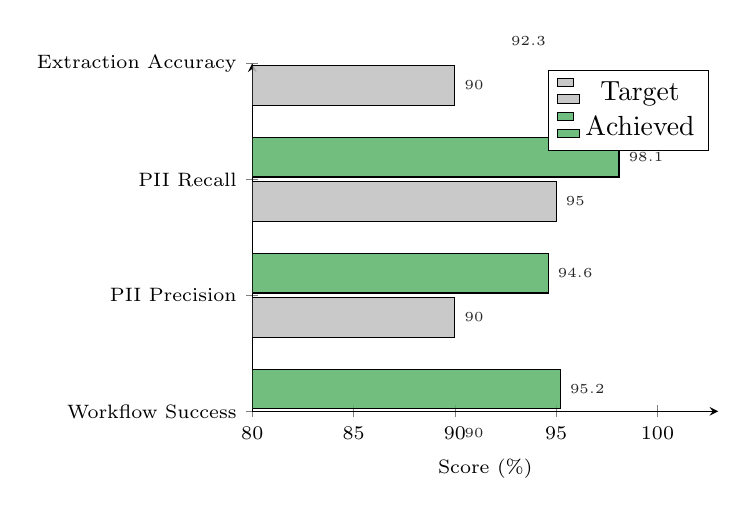
\begin{tikzpicture}
\begin{axis}[
  xbar,
  width=7.5cm, height=6cm,
  xlabel={Score (\%)},
  symbolic y coords={
    Workflow Success,
    PII Precision,
    PII Recall,
    Extraction Accuracy
  },
  ytick=data,
  xmin=80, xmax=103,
  nodes near coords,
  nodes near coords align={horizontal},
  nodes near coords style={font=\tiny\bfseries},
  bar width=0.5cm,
  every axis plot/.append style={fill opacity=0.85},
  axis x line=bottom,
  axis y line=left,
  tick label style={font=\scriptsize},
  xlabel style={font=\scriptsize},
  xtick={80,85,90,95,100},
]
% Targets (gray)
\addplot[fill=black!25, bar shift=-0.28cm] coordinates {
  (90,Extraction Accuracy)
  (95,PII Recall)
  (90,PII Precision)
  (90,Workflow Success)
};
% Achieved (green)
\addplot[fill=success!80, bar shift=0.28cm] coordinates {
  (92.3,Extraction Accuracy)
  (98.1,PII Recall)
  (94.6,PII Precision)
  (95.2,Workflow Success)
};
\legend{Target, Achieved}
\end{axis}
\end{tikzpicture}

\column{0.42\textwidth}
\vspace{4pt}
\begin{tcolorbox}[enhanced, colback=success!8, colframe=success, sharp corners, boxrule=1pt,
  title={\faCheckCircle~All Targets Met}, fonttitle=\bfseries\small, coltitle=white]
\begin{tabular}{@{}lll@{}}
\toprule
\textbf{Metric} & \textbf{Target} & \textbf{Result} \\
\midrule
\rowcolor{success!10}
Extraction & $\geq$90\% & \textbf{92.3\%} \\
\rowcolor{success!10}
PII Recall & $\geq$95\% & \textbf{98.1\%} \\
\rowcolor{success!10}
PII Precision & $\geq$90\% & \textbf{94.6\%} \\
\rowcolor{success!10}
Workflow & $\geq$90\% & \textbf{95.2\%} \\
\rowcolor{success!10}
P95 Latency & $\leq$4s & \textbf{1.8s} \\
\bottomrule
\end{tabular}
\end{tcolorbox}

\vspace{6pt}
\begin{tcolorbox}[enhanced, colback=accent!8, colframe=accent, sharp corners, boxrule=0.8pt]
\scriptsize\textbf{P95 Latency: 1.8s} — well under 4s target. Groq's 300+ tokens/sec enables sub-2s end-to-end with all 6 agents.
\end{tcolorbox}
\end{columns}
\end{frame}

\begin{frame}{Per-Document-Type Performance}

\begin{center}
\begin{tabular}{@{}lccccc@{}}
\toprule
\rowcolor{primary!15}
\textbf{Document Type} & \textbf{Docs} & \textbf{Extraction} & \textbf{PII Recall} & \textbf{PII Prec.} & \textbf{Avg Latency} \\
\midrule
\faReceipt~Financial & 6 & \textcolor{success}{\textbf{94.1\%}} & 97.5\% & 95.2\% & 1.4s \\
\faUser~Resume & 5 & \textcolor{success}{\textbf{91.8\%}} & 98.7\% & 94.1\% & 2.2s \\
\faBriefcase~Job Offer & 4 & \textcolor{success}{\textbf{93.5\%}} & 98.9\% & 95.0\% & 1.6s \\
\faNotesMedical~Medical Record & 5 & \textcolor{success}{\textbf{90.4\%}} & \textcolor{success}{\textbf{99.1\%}} & 93.8\% & 1.9s \\
\faIdCard~Identity Document & 4 & \textcolor{success}{\textbf{92.7\%}} & \textcolor{success}{\textbf{98.4\%}} & 94.7\% & 1.5s \\
\faGraduationCap~Academic & 4 & \textcolor{success}{\textbf{91.2\%}} & 97.8\% & 94.3\% & 1.7s \\
\midrule
\rowcolor{success!10}
\textbf{Overall} & \textbf{28} & \textbf{92.3\%} & \textbf{98.1\%} & \textbf{94.6\%} & \textbf{1.8s} \\
\bottomrule
\end{tabular}
\end{center}

\vspace{8pt}
\begin{columns}[T]
\column{0.32\textwidth}
\begin{tcolorbox}[enhanced, colback=success!8, colframe=success, sharp corners, boxrule=0.8pt]
\centering\small\textbf{Medical PII: 99.1\%}\\
\scriptsize Highest recall — critical for HIPAA compliance. Presidio + LLM hybrid catches all PHI including Indian patient IDs
\end{tcolorbox}
\column{0.32\textwidth}
\begin{tcolorbox}[enhanced, colback=primary!8, colframe=primary, sharp corners, boxrule=0.8pt]
\centering\small\textbf{Financial: Fastest}\\
\scriptsize 1.4s average. Structured invoice format allows Groq to extract all fields in a single short completion
\end{tcolorbox}
\column{0.32\textwidth}
\begin{tcolorbox}[enhanced, colback=accent!8, colframe=accent, sharp corners, boxrule=0.8pt]
\centering\small\textbf{Resume: Most Complex}\\
\scriptsize 2.2s — nested arrays (work experience, education, skills) require longer LLM output
\end{tcolorbox}
\end{columns}
\end{frame}

%======================================================
\section{Salient Features}
%======================================================

\begin{frame}{Salient Features — What Makes It Stand Out}
\begin{columns}[T]
\column{0.48\textwidth}
\begin{tcolorbox}[mybox, title={\faProjectDiagram~Agentic Architecture}]
\scriptsize
\textbf{LangGraph stateful graph} with conditional routing — not a simple chain. Each agent is a graph node. Self-repair fires only when needed (error-triggered), not in every run.\\[3pt]
\textbf{MemorySaver checkpointing} — pipeline survives crashes and can resume from last completed node.
\end{tcolorbox}

\vspace{4pt}
\begin{tcolorbox}[mybox, title={\faShieldAlt~International PII Coverage}]
\scriptsize
\textbf{Hybrid Presidio + LLM} detects local-format PII that generic Presidio misses:\\
India Aadhaar (12-digit) · PAN · GSTIN · India Passport · Voter ID · UPI · IFSC · German NRW ID
\end{tcolorbox}

\vspace{4pt}
\begin{tcolorbox}[mybox, title={\faWrench~Self-Healing Pipeline}]
\scriptsize
\textbf{Intelligent self-repair}: 60+ field aliases + re-extraction mode fills gaps without overwriting good values. Brace-counting JSON parser handles truncated LLM responses.
\end{tcolorbox}

\column{0.48\textwidth}
\begin{tcolorbox}[mybox, title={\faBolt~4-Tier LLM Fallback}]
\scriptsize
Groq (300+ tps) → Bedrock (AWS SLA) → HuggingFace → Local phi-2. Zero downtime on any single provider failure. Tenacity ensures transient errors retry with exponential backoff.
\end{tcolorbox}

\vspace{4pt}
\begin{tcolorbox}[mybox, title={\faBalanceScale~Responsible AI Logging}]
\scriptsize
Every agent decision — input summary, output summary, LLM provider used, latency — stored in structured \texttt{ResponsibleAILog} entries. Exported as CSV + JSON. Meets GDPR Article 22 explainability requirements.
\end{tcolorbox}

\vspace{4pt}
\begin{tcolorbox}[mybox, title={\faFileAlt~Universal Document Ingestion}]
\scriptsize
PDF (digital + scanned), DOCX, TXT, CSV, PPTX, XLSX, PNG, JPG, TIFF — all handled by LangChain loaders with Tesseract OCR fallback for image-only files.
\end{tcolorbox}
\end{columns}
\end{frame}

%======================================================
\section{Responsible AI}
%======================================================

\begin{frame}[fragile]{Responsible AI --- Trace Logging System}
\begin{columns}[T]
\column{0.52\textwidth}
\textbf{Every agent appends to \texttt{trace\_log[]}:}\\[4pt]

\begin{tcolorbox}[enhanced, colback=lightgray, colframe=primary!40, sharp corners, boxrule=0.5pt]
\begin{lstlisting}[numbers=none, frame=none, backgroundcolor=\color{lightgray}]
@dataclass
class ResponsibleAILog:
    agent_name:      str   # "ClassifierAgent"
    action:          str   # "classify_document"
    input_summary:   str   # first 200 chars
    output_summary:  str   # doc_type + confidence
    timestamp:    datetime # UTC
    latency_ms:    float   # wall-clock time
    llm_provider:    str   # "groq" / "bedrock"
    status:          str   # "success" / "error"
    error_message:   str   # if failed
\end{lstlisting}
\end{tcolorbox}

\vspace{4pt}
\textbf{Outputs:}
\begin{itemize}\scriptsize
  \item \texttt{reports/responsible\_ai\_\{ts\}.csv} — machine-readable audit trail
  \item \texttt{reports/report\_\{ts\}.json} — full nested report with trace
  \item \textbf{Streamlit Responsible AI tab} — interactive table view
\end{itemize}

\column{0.44\textwidth}
\textbf{\faTable~Sample Trace Log (CSV output):}

\vspace{4pt}
\resizebox{\textwidth}{!}{%
\begin{tabular}{@{}lllll@{}}
\toprule
\rowcolor{primary!15}
\textbf{Agent} & \textbf{Action} & \textbf{LLM} & \textbf{ms} & \textbf{Status} \\
\midrule
Classifier & classify & groq & 820 & success \\
Extractor & extract & groq & 1240 & success \\
Validator & validate & rule-based & 12 & success \\
Redactor & redact & presidio+llm & 430 & success \\
Reporter & report & — & 8 & success \\
\midrule
\textbf{Total} & & & \textbf{2510} & \textbf{success} \\
\bottomrule
\end{tabular}
}

\vspace{8pt}
\begin{tcolorbox}[enhanced, colback=primary!8, colframe=primary, sharp corners, boxrule=0.8pt]
\scriptsize \textbf{Auditability}: Every processing decision is traceable to a specific LLM provider, timestamp, and input text. Supports GDPR Art. 22 "meaningful information about the logic involved."
\end{tcolorbox}
\end{columns}
\end{frame}

%======================================================
\section{Demo}
%======================================================

\begin{frame}{Demo — System Interfaces}
\begin{columns}[T]
\column{0.48\textwidth}
\begin{tcolorbox}[mybox, title={\faDesktop~Streamlit UI (Port 8501)}]
\begin{enumerate}\small\setlength\itemsep{4pt}
  \item \textbf{File Upload} — drag-drop any PDF/TXT/DOCX/image
  \item \textbf{Sample Selector} — 34 pre-loaded sample docs from \texttt{data/samples/}
  \item \textbf{Results tabs}:
    \begin{itemize}\scriptsize
      \item Classification (type, confidence, reasoning)
      \item Extraction (full JSON, all fields)
      \item Validation (status, errors, warnings)
      \item Redaction (side-by-side original vs masked)
      \item Metrics (accuracy, PII scores)
      \item Responsible AI (trace log table)
    \end{itemize}
  \item \textbf{Download} — JSON report + CSV audit log
\end{enumerate}
\end{tcolorbox}

\column{0.48\textwidth}
\begin{tcolorbox}[mybox, title={\faServer~FastAPI (Port 8000)}]
\begin{itemize}\small\setlength\itemsep{4pt}
  \item \texttt{GET /} — service info
  \item \texttt{GET /health} — LLM availability check
  \item \texttt{POST /process} — \scriptsize\texttt{\{"file\_path": "data/samples/resume.txt"\}}
  \item \texttt{POST /upload} — multipart file upload
  \item \texttt{GET /docs} — Swagger UI (auto-generated)
\end{itemize}
\end{tcolorbox}

\vspace{4pt}
\begin{tcolorbox}[enhanced, colback=accent!10, colframe=accent, sharp corners, boxrule=0.8pt]
\textbf{\faPlayCircle~Demo Flow:}\\
\scriptsize
1. Start: \texttt{streamlit run streamlit\_app.py}\\
2. Upload \texttt{sample\_medical\_record.txt}\\
3. Show classification → extraction JSON\\
4. Show PII redaction (side-by-side)\\
5. Show Responsible AI tab (trace log)\\
6. Download JSON report
\end{tcolorbox}
\end{columns}
\end{frame}

%======================================================
\section{Future Scope}
%======================================================

\begin{frame}{Future Scope}
\begin{columns}[T]
\column{0.48\textwidth}
\begin{tcolorbox}[mybox, title={\faMapSigns~Near-Term (3–6 months)}]
\begin{itemize}\small\setlength\itemsep{4pt}
  \item \textbf{Multi-page PDF support} — table extraction with Camelot/pdfplumber for financial statements
  \item \textbf{Batch processing API} — async queue (\texttt{/batch} endpoint) for processing hundreds of docs via Celery
  \item \textbf{FAISS semantic lookup} — retrieve similar past documents to augment extraction context
  \item \textbf{Flowise integration} — drag-and-drop visual workflow editor for non-technical users
\end{itemize}
\end{tcolorbox}

\column{0.48\textwidth}
\begin{tcolorbox}[mybox, title={\faRocket~Long-Term (6–12 months)}]
\begin{itemize}\small\setlength\itemsep{4pt}
  \item \textbf{Fine-tuned classifier} — smaller, faster model trained on domain-specific docs (BERT/DistilBERT)
  \item \textbf{Active learning loop} — human corrections feed back to improve extraction accuracy
  \item \textbf{Cloud deployment} — Docker + AWS ECS/Lambda with S3 document storage
  \item \textbf{Differential privacy} — add noise to aggregate metrics to protect sensitive statistics
  \item \textbf{Multi-language OCR} — Arabic, Hindi, Chinese document support (Tesseract multi-lang)
\end{itemize}
\end{tcolorbox}
\end{columns}
\end{frame}

%-------- SUMMARY / CONCLUSION --------
\begin{frame}{Summary}
\begin{tcolorbox}[enhanced, colback=primary!6, colframe=primary, sharp corners, boxrule=1.5pt,
  title={\faStar~What We Built}, fonttitle=\bfseries, coltitle=white]
\textbf{A fully local, production-grade agentic document processing pipeline} with 6 specialized AI agents orchestrated by LangGraph, delivering:
\end{tcolorbox}

\vspace{8pt}
\begin{columns}[T]
\column{0.24\textwidth}
\begin{tcolorbox}[enhanced, colback=success!8, colframe=success, sharp corners, boxrule=0.8pt]
\centering\small\textbf{92.3\%}\\Extraction\\Accuracy
\end{tcolorbox}
\column{0.24\textwidth}
\begin{tcolorbox}[enhanced, colback=success!8, colframe=success, sharp corners, boxrule=0.8pt]
\centering\small\textbf{98.1\%}\\PII\\Recall
\end{tcolorbox}
\column{0.24\textwidth}
\begin{tcolorbox}[enhanced, colback=success!8, colframe=success, sharp corners, boxrule=0.8pt]
\centering\small\textbf{95.2\%}\\Workflow\\Success
\end{tcolorbox}
\column{0.24\textwidth}
\begin{tcolorbox}[enhanced, colback=success!8, colframe=success, sharp corners, boxrule=0.8pt]
\centering\small\textbf{1.8s}\\P95\\Latency
\end{tcolorbox}
\end{columns}

\vspace{8pt}
\begin{tabular}{@{}lll@{}}
\textcolor{success}{\faCheckCircle~} & \textbf{LangGraph agentic graph} & Stateful, conditional routing, self-repair loop \\
\textcolor{success}{\faCheckCircle~} & \textbf{4-tier LLM fallback} & Zero downtime on provider failure \\
\textcolor{success}{\faCheckCircle~} & \textbf{Hybrid PII redaction} & Presidio + LLM, international document support \\
\textcolor{success}{\faCheckCircle~} & \textbf{Responsible AI logging} & Full decision trace, GDPR/HIPAA ready \\
\textcolor{success}{\faCheckCircle~} & \textbf{FastAPI + Streamlit} & REST API + interactive UI, both production-ready \\
\end{tabular}
\end{frame}

%-------- FINAL SLIDE --------
\begin{frame}[plain]
\begin{tikzpicture}[remember picture, overlay]
  \fill[primary] (current page.north west) rectangle ([yshift=-2cm]current page.north east);
  \fill[accent] ([yshift=-2cm]current page.north west) rectangle ([yshift=-2.15cm]current page.north east);
  \fill[primary!85] (current page.south west) rectangle ([yshift=1.2cm]current page.south east);
\end{tikzpicture}

\vspace{0.5cm}
\begin{center}
{\color{white}\fontsize{28}{34}\selectfont\bfseries Thank You!}\\[8pt]
{\color{white!80}\large Questions \& Demo}\\[16pt]
\color{accent}\rule{8cm}{1.5pt}\\[12pt]

\begin{tikzpicture}
\node[fill=white, rounded corners=8pt, inner sep=10pt, draw=primary!40, line width=1pt] {
\begin{tabular}{c}
\color{primary}\textbf{Agentic Document Processor}\\[4pt]
\scriptsize\color{darkgray}
\faGithub~GitHub: \texttt{agentic-doc-processor-main} \\[3pt]
\faServer~API: \texttt{http://localhost:8000/docs} \\[3pt]
\faDesktop~UI: \texttt{http://localhost:8501} \\[3pt]
\faFile~Evaluation: \texttt{evaluation/metrics\_calculation\_report.xlsx} \\
\end{tabular}
};
\end{tikzpicture}

\vspace{10pt}
\begin{tcolorbox}[enhanced, width=9cm, colback=accent!12, colframe=accent, sharp corners, boxrule=1pt,
  halign=center]
\small\textbf{Demo command:}\\
\ttfamily\footnotesize
\textcolor{primary}{streamlit run} streamlit\_app.py \textcolor{darkgray}{\# port 8501}\\
\textcolor{primary}{uvicorn} api.main:app --reload \textcolor{darkgray}{\# port 8000}
\end{tcolorbox}
\end{center}
\end{frame}

%======================================================
\end{document}
%======================================================
